
% =============================================================================
% =============================================================================
% =============================================================================
\section{Finite Poloidal Lifetimes}
  \label{sec_lifetimes}

Radoski\cite{radoski_1974} looked at \Alfven waves, using a cylindrical coordinate system to imitate an ``unwrapped'' dipole. He argued that poloidal waves should asymptotically rotate to the toroidal mode. 

Mann\cite{mann_1995} performed some wave-in-a-box simulations and found the rotation time to be linear in modenumber: $\tau = \frac{d \lambda}{d \omega_A'}$, where $\lambda = \frac{\azm}{2 \pi r}$ and $\omega_A'$ is the spatial derivative of the \Alfven bounce frequency. Soon afterwards\cite{mann_1997}, he supported his simulations analytically. 

\todo{Crunch out $\frac{d \lambda}{d \omega_A'}$. Preliminary indications are that it doesn't translate well to a realistic grid, but let's double check. }

Ding\cite{ding_1995} ran simulations more-or-less concurrent with Mann's. Ding saw a rotation from poloidal to toroidal... then back again. It seems that the reversal was a spatial resolution issue. 

The aforementioned models made significant simplifying assumptions in terms of geometry and boundary conditions. 

Mann used straight field lines, a uniform \Alfven speed gradient, and perfectly conducting boundaries. 

Ding's simulation is nominally carried out in a dipole geometry, but the ionospheric boundary is at \SI{2.5}{\RE}. Boundaries are also perfectly conducting. 

That is, the results below offer a significantly higher level of realism than any past simulation (in part, of course, because computers are a lot better than they were 20 years ago). 

A dedicated 3D treatment of this problem is unlikely at present. Large azimuthal modenumbers are expensive to compute. That's the whole point! 

The energy is obtained by integrating (using the Jacobian to handle the grid properly) $U = \int dU = \int u \, dV$. Values are the log (base 10) of that, in the slightly odd units of gigajoules per radian. A factor of $2\pi$ wouldn't change anything, of course, but it seems inappropriate to integrate all the way around the sphere when Pc4s are longitudinally localized (a fact which was an important part of justifying a 2.5D approach). 

% -----------------------------------------------------------------------------
% -----------------------------------------------------------------------------
% -----------------------------------------------------------------------------
\subsection{High Conductivity}

In \cref{fig_U_day}, the rotation of energy from the poloidal mode to the toroidal mode is clear. Driving is strictly poloidal, yet the toroidal mode accumulates energy over time, and doesn't appear to give it back. The rotation happens faster for low-\azm simulations, qualitatively consistent with Mann's result; the time at which poloidal and toroidal energies are equal seems to even be linear in \azm, in line with his result. 

At least, this is the case on the dayside, where the ionosphere is highly conductive. 

\begin{figure}[H]
    \centering
    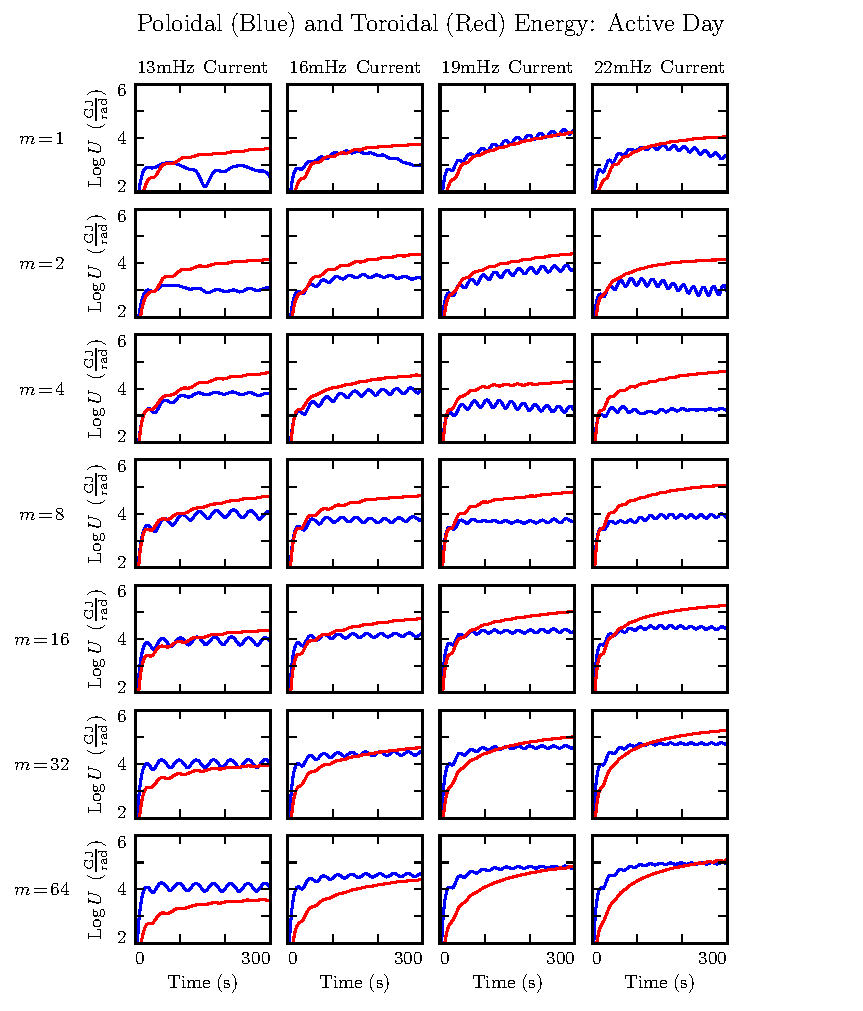
\includegraphics[width=\textwidth]{figures/U_1.pdf}
    \caption[Poloidal and Toroidal Energy: Active Day]{
      Driving -- delivered to the poloidal mode -- asymptotically rotates to the toroidal mode. The rate of rotation is strongly affected by the azimuthal modenumber. 
    }
    \label{fig_U_day}
\end{figure}

\todo{Talk about why this is exciting. }

\todo{Note that Mann looked specifically at second-harmonic waves. }

\todo{This result shows agreement with -- and significant refinement of -- Mann's findings. In the case of large-but-finite ionospheric conductivity, dipole geometry, and realistic \Alfven speed profile, energy does asymptotically rotate from the poloidal mode to the toroidal mode. The rotation rate is strongly affected by azimuthal modenumber and, in the case of large-but-finite \azm, has a characteristic timescale in the tens of periods. The present work furthermore demonstrates that the rotation rate is affected by driving frequency (did Mann talk about this at all, or just work in normalized time?) }

% -----------------------------------------------------------------------------
% -----------------------------------------------------------------------------
% -----------------------------------------------------------------------------
\subsection{Low Conductivity}

The picture on the nightside (where the ionospheric conductivity is low) is significantly different from the dayside (where it's high). 

Dissipation seems to outstrip rotation. Energy does not accumulate over numerous driving periods, as would be expected in resonance; it follows the driving up and down, as a damped-driven oscillator. 

There is evidence that the rotation is still trying to happen. At low \azm, energy is distributed between the poloidal and toroidal mode before dissipating; at high \azm, the energy dissipates straight out of the poloidal mode, never having had a chance to rotate. 

\begin{figure}[H]
    \centering
    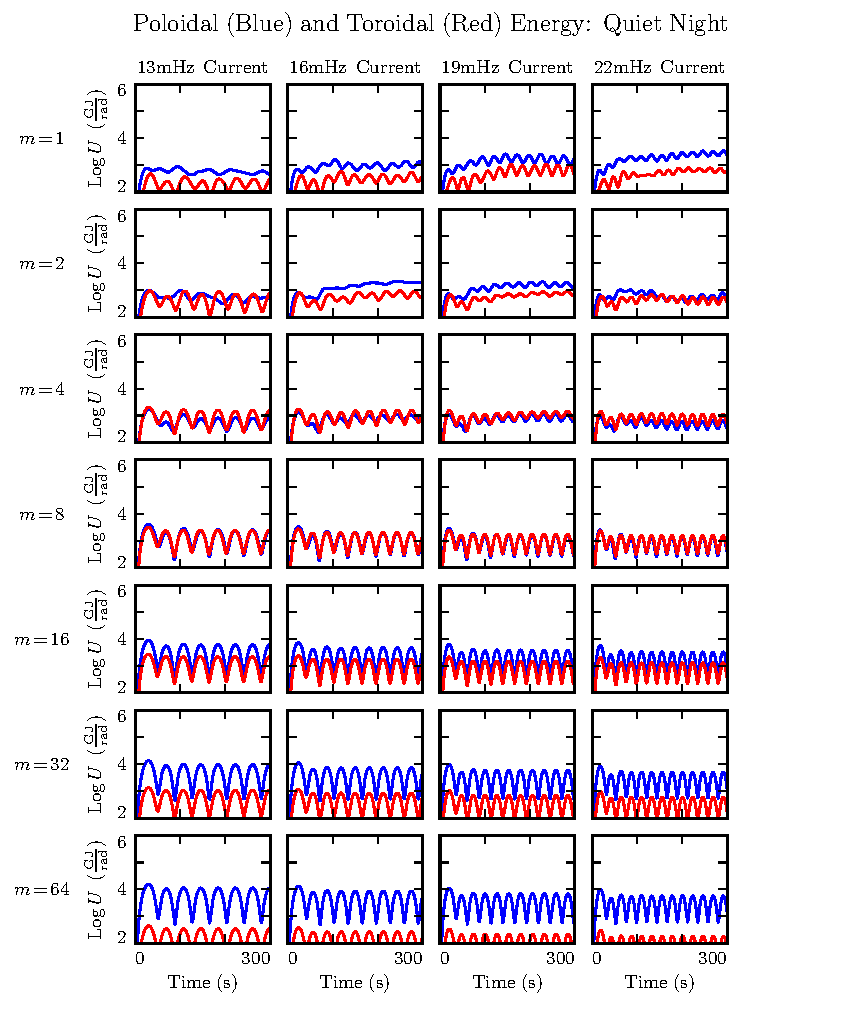
\includegraphics[width=\textwidth]{figures/U_4.pdf}
    \caption[Poloidal and Toroidal Energy: Quiet Night]{
      Driving is applied to the poloidal electric field. There is some rotation of energy to the toroidal mode (and less at high azimuthal modenumber), but the low ionospheric conductivity prevents energy from accumulating over time. 
    }
    \label{fig_U_night}
\end{figure}

\todo{Why is this exciting? }

\todo{Previous considerations of poloidal lifetimes have been limited to the high conductivity regime. The present work demonstrates that the low conductivity regime exhibits qualitative differences. Ionospheric conductivity on the nightside is low enough that resonance does not develop, even in the case of ongoing driving. The dissipation timescale is comparable to the rotation timescale. Rather than aymoptotically accumulating energy in the toroidal mode, the oscillator asymptotically oscillates following the driving. This is relevant to the question of day-night asymmetry in the observation of field line resonances. }

